\newpage
\section{Tree}

一个基本的 Tree 如下图所示:

\begin{figure}[H]
    \centering
    \begin{minipage}{0.35\linewidth}
        \centering
        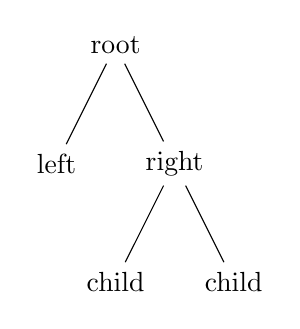
\begin{tikzpicture}[scale = 1]
            \node {root}
                child {node {left}}
                child {node {right}
                    child {node {child}}
                    child {node {child}}
            };
        \end{tikzpicture}
    \end{minipage}
    \begin{minipage}{0.55\linewidth}
        \begin{lstlisting}[style = latex-side]
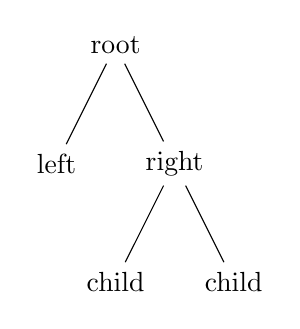
\begin{tikzpicture}[scale = 1]
    \node {root}
        child {node {left}}
        child {node {right}
            child {node {child}}
            child {node {child}}
    };
\end{tikzpicture}
        \end{lstlisting}
    \end{minipage}
    \caption{TikZ 基础树}
\end{figure}

\begin{itemize}
    \item child 关键字
    
    树的根节点下跟着 child 关键字即可构建树,其中 child 的语法如下:

    \begin{lstlisting}[style = latex]
    \path … child [<options>] foreach <variables> in {<values>} {<child path>} …;
    \end{lstlisting}

    其中, \texttt{foreach} 用于创建当前节点下的多个子结点。下面两种写法效果是相同的
    \begin{figure}[H]
        \centering
        \begin{minipage}{0.8\linewidth}
            \begin{lstlisting}[style = latex-side]
    % 没有样式的 foreach
    node {root} child [red] foreach \name in {1,2} {node {\name}}
    node {root} child [red] {node {1}} child[red] {node {2}}
    % 带样式的 foreach
    node {root} child[\pos] foreach \name/\pos in {1/left,2/right} {node[\pos] {\name}}
    node {root} child[left] {node[left] {1}} child[right] {node[right] {2}}
            \end{lstlisting}
        \end{minipage}
        \caption{child 节点的 foreach}
    \end{figure}
\end{itemize}

